\begin{quote}
  This chapter develops the idea that comprehensive scene
  understanding at the level of objects, actions, and surfaces
  requires at least a rudimentary understanding of the high--level
  geometry of the environment. There are many ways to capture such
  coarse geometry; here we argue that the indoor Manhattan
  representation is an excellent choice in terms of the salient
  geometric information it captures, its simplicity, and the elegant
  inference procedures it permits. This chapter focusses on analysing
  the model itself, leaving algorithms and empirical results to later
  chapters. This constitutes the first comprehensive definition and
  analysis of indoor Manhattan environments in the literature (though
  not the first account \textit{per se} \cite{Lee09}). The primary
  contributions of this chapter are a derivation of the ``vertex'' and
  ``seam'' parametrisations, and the description of several properties
  of these parametrisations that will prove crucial to the development
  of the following chapters.\footnotemark
\end{quote}

\footnotetext{
{ \setlength{\parindent}{0pt} 
  This work was published in part in:\\
  \textit{Flint, Mei, Murray, and Reid,} ``A Dynamic Programming
  Approach To Reconstruction Building Interiors'', in \textit{Proceedings
    of the 2010 European Conference on Computer Vision}\quad\cite{Flint10eccv}
}
}

\begin{figure}[tb]%
  \centering
    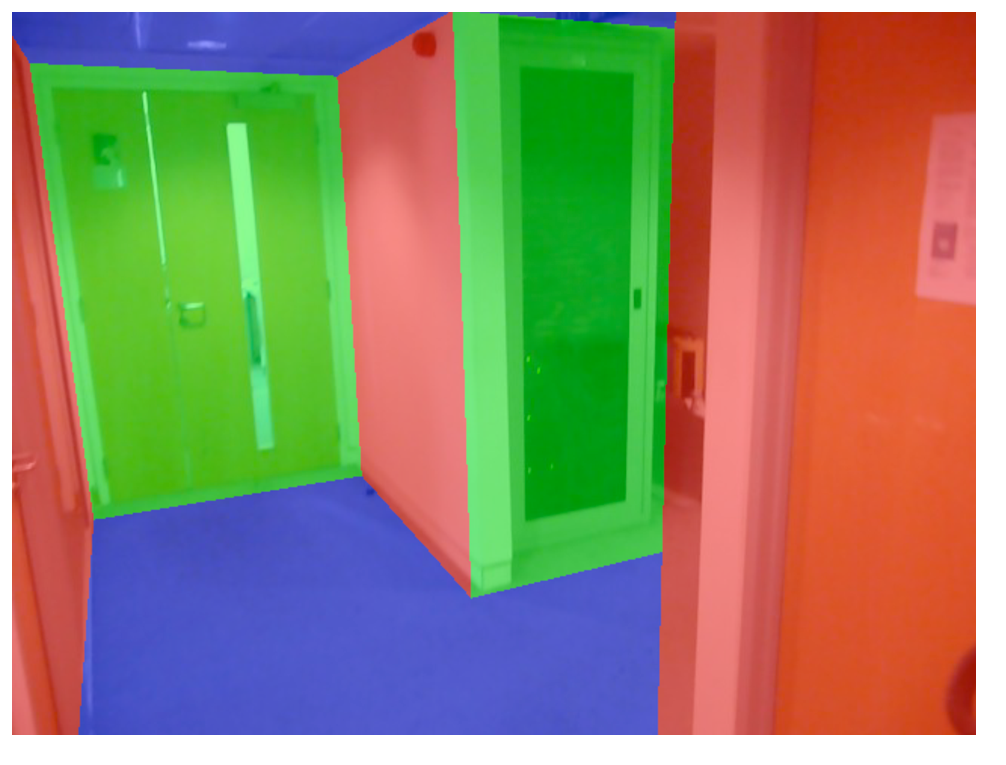
\includegraphics[width=0.45\textwidth]{manhattan-eg2}
    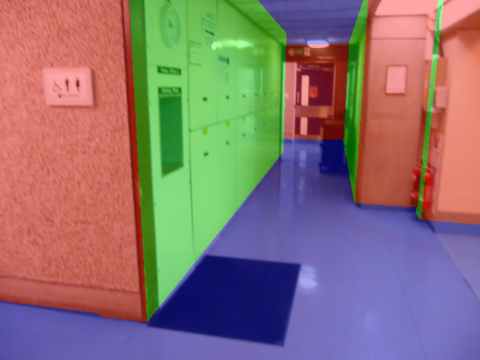
\includegraphics[width=0.45\textwidth]{manhattan-eg1.png}
    \caption{Two examples of indoor Manhattan environments.}
  \label{fig:geometry-egs}
\end{figure}

%%%%%%%%%%%%%%%%%%%%%%%%%%%%%%%%%%%%%%%%%%%%%%%%%%%%%%%%%%%%%%%%%%%%%%%%
\section{Introduction}

The preceding chapter described an approach to scene understanding in
which raw image features were connected directly to high--level
quantities such as scene categories. This chapter begins the
development of a more sophisticated model in which pixel--level
features are connected to high--level quantities via an unobserved
intermediate level representing scene geometry. We focus on recovering
this intermediate representation, leaving the application to specific
classification tasks to future work. There are a number of reasons to
see geometry as central to scene understanding. For an intuitive
demonstration, consider the information conveyed by the red, green,
and blue regions in \figref{geometry-egs}. These regions have very low
fidelity (the entire model is defined by just a handful of polygons),
yet it is clear that they convey considerable information about the
likely locations of various objects, the scale at which those objects
would appear, and how they would interact.

There are many choices for the representation of the
intermediate--level variables; the following desiderata summarise the
requirements relevant to our goals.
\begin{enumerate}
  \item{\textbf{Salience.} Of all the information present at the
    image level, the intermediate variables should capture as much of
    the information that is \textit{relevant} to inferring the
    high--level quantities of interest as possible.}
  \item{\textbf{Compression.} The intermediate representation should
    discard as much irrelevant information as possible. All else
    equal, we prefer succinct representations of the world for
    efficiency reasons. See MacKay \cite{MacKay2003} for a discussion
    of the connection between compression and learning.}
  \item{\textbf{Tractability.} All else equal, we prefer
    representations that lead to simple and efficient inference
    algorithms. A simple model for which inference is tractable
    may be preferable to a slightly more expressive model in which
    one must rely on approximate inference procedures with
    poorly--understood convergence properties.}
  \item{\textbf{Simplicity.} All else equal, we prefer representations
    consisting of quantities that are intuitive to humans.}
  \item{\textbf{Generality.} The chosen representation should be
    applicable to a wide variety of real--world environments.}
\end{enumerate}

We have chosen to work with the indoor Manhattan representation, in
which the world is built up from a floor plane, a ceiling plane, and a
sequence of vertical wall segments. This representation was originally
proposed by Lee \etal \cite{Lee09}. Indoor Manhattan environments are
a sub--class of general Manhattan environments, which simply specify
surfaces in three mutually orthogonal directions. Indoor Manhattan
scenes satisfy the desiderata above for the following reasons.
\begin{itemize}
  \item{\textbf{Compression and salience.} As described above, the
    geometric entities present in the indoor Manhattan representation
    correlate well the high--level quantities of interest for scene
    understanding. The models shown in \figref{geometry-egs} consume
    just a few hundred bytes, yet capture much of the information
    present in the original image data, which consumes three orders of
    magnitude more space. The point here is not to save disk space,
    but to demonstrate that indoor Manhattan models efficiently capture
    salient information.}
  \item{\textbf{Simplicity.} Iindoor Manhattan models are composed of
    quantities that have 
    have natural semantics, being associated with entities such as the
    floor, walls, and ceiling of an environment.}
  \item{\textbf{Generality.} Indoor Manhattan models can represent
    many environments exactly or approximately; even those that do not
    conform exactly to the assumptions of the model. We expand on this later.}
  \item{\textbf{Tractability.} Indoor Manhattan scenes have special
    geometric structure that permits an elegant ``seam''
    representation. This in term leads to efficient and exact
    inference algorithms for a range of sensor models, and an
    attractive learning algorithm. This are the subject of the ensuing
    chapters.}
\end{itemize}

By adopting the indoor Manhattan representation we are \textit{not}
restricted to working with \textit{ideal} indoor Manhattan
environments --- environments free of clutter, occlusions, windows,
or other deviations from our assumptions. Rather, the point is to take
account of such deviations in the probabilistic model relating image
features to scene structure. For example, the model we present for
depth measurements in \chapref{inference} explicitly marginalises over
the possibility that a given depth measurement corresponds to a
clutter object, an object observed through a window, or an erroneous
measurement. Thus we cast the Manhattan scene geometry as a latent
variable to be inferred in the presence of noise, clutter, and
occlusions, rather than as a complete description of everything we
might observe. Empirical results in forthcoming chapters show many
examples of our system working in real--world environments that are
very far from ideal indoor Manhattan scenes, containing poor lighting
and noisy images in addition to clutter, windows, and
non--Manhattan--aligned surfaces.

However, this chapter focusses on analysing the representation itself,
and so is concerned with ideal indoor Manhattan scenes. The
contributions of this chapter are (1) the first comprehensive
definition of the indoor Manhattan assumption; (2) two novel
representations for indoor Manhattan scenes; and (3) a number of minor
results connecting these representations and providing other insights
crucial to the ensuing chapters. As mentioned above, this chapter does
not contain any experimental results, though it does provide the
conceptual infrastructure that the remainder of this thesis builds
on. We begin by defining indoor Manhattan scenes, then we discuss our
first representation in terms of floorplans, followed a description of
the ``vertex'' and ``seam'' parametrisations that will be used in
following chapters. \secref{misc-geometry} contains a number of minor
deductions of relevance to the ensuing chapters, then we close with a
brief conclusion.

%%%%%%%%%%%%%%%%%%%%%%%%%%%%%%%%%%%%%%%%%%%%%%%%%%%%%%%%%%%%%%%%%%%%%%%%
\section{Indoor Manhattan Environments}

Let a reconstruction $\Reconstruction$ consist of a set of polygons
$\Poly_i$ with vertices $\vertex_j\in\Rthree$. An \textit{indoor
  Manhattan reconstruction} is a reconstruction $\Reconstruction$ with
the following properties.
\begin{enumerate}
\item{\textit{Each polygon is oriented in one of three mutually
    orthogonal directions}. Formally, for each pair of polygons
  $\Poly_i,\Poly_j \in \Reconstruction$ with unit--length normals
  $\normal_i,\normal_j$,
  \begin{equation}
    \normal_i \cdot \normal_j \in \{0,1\}
  \end{equation}
}
\item{\textit{There is a floor plane and a ceiling plane}. Formally,
  there exists some direction $\vertnormal$ and a pair of real
  numbers $\zfloor, \zceil$ such that each polygon
  $P\in\Reconstruction$ with normal $\normal=\vertnormal$ has
  vertices $\vertex$ satisfying
  \begin{equation}
    \vertex \cdot \vertnormal \in \{\zfloor, \zceil\}
  \end{equation}
}
\item{\textit{Vertical walls extend from floor to ceiling}. Formally, if
  $\normal_i \neq \vertnormal$ then we say that $\Poly_i \in
  \Reconstruction$ is a \textit{vertical} polygon. This
  condition is satisfied if and only if each vertex $\vertex$ of
  each vertical polygon satisfies
  \begin{equation}
    \vertex \cdot \vertnormal \in \{\zfloor, \zceil\}
  \end{equation}
}
\item{\textit{The edges of walls are vertical}. Formally, if
  $\vertex\in\Poly$ and $\vertex\cdot\vertnormal=\zfloor$, then
  $\exists\othervertex\in\Poly$ such that
  \begin{equation}
    \othervertex \cdot \vertnormal = \zceil
  \end{equation}
  and
  \begin{equation}
    \othervertex = \vertex + \ScaleParam \vertnormal
  \end{equation}
  for some $\ScaleParam \in \Reals$.
}
\end{enumerate}

We assume a pinhole camera mapping homogeneous world coordinates
$\vect{X}\in\Rfour$ to homogeneous image coordinates $\vect{x}\in\Rthree$
according to
\begin{equation}
  \vect{x} = 
  \CamMatrix \begin{bmatrix} \CamR & \CamTr \end{bmatrix} \vect{X} ~,
\end{equation}
where $\CamMatrix$ is a $3 \times 3$ homography, $\CamR$ is a
3--dimensional rotation matrix, and $\CamTr$ is a 3--dimensional
translation.

We define an indoor Manhattan \textit{scene} as a reconstruction
together with a camera viewpoint, subject to the following additional
constraints.
\begin{enumerate}
  \item{The camera centre $\vect{c}$ is located between the floor
    and ceiling planes,
    \begin{equation}
      \zfloor < \vect{c} \cdot \vertnormal < \zceil
    \end{equation}
  }
  \item{The reconstruction is closed relative to the camera
    viewpoint. Formally, for each viewing direction $\vect{x}$ there
    is some polygon $\Poly\in\Reconstruction$ containing a point
    $\vect{X}$ that projects to $\vect{x}$.
  }
\end{enumerate}

In general we will assume that scenes consist only of those polygons
visible to the camera. Since reconstructions consists of a finite
number of polygons and our camera model is linear, it can be shown
that an indoor Manhattan reconstruction truncated to a view
frustum remains an indoor Manhattan reconstruction as defined
above.

%%%%%%%%%%%%%%%%%%%%%%%%%%%%%%%%%%%%%%%%%%%%%%%%%%%%%%%%%%%%%%%%%%%%%%%%
\section{Floorplans}

The polygonal representation for indoor Manhattan environments is
inconvenient for our purposes. A more useful representation is a
\textit{floorplan}, in which walls are represented as line segments
in the $XY$ plane. Formally, we define a floorplan $\Floorplan$ as a
tuple $(\SceneR,\Zs,\Polyline)$, where
\begin{itemize}
  \item{$\SceneR$ is a 3--dimensional rotation;}
  \item{$\Zs=(\zfloor,\zceil)$ is a pair of scalars defining the floor
    and ceiling planes,
    \begin{eqnarray}
      \Pfloor &=& \{ \vect{x} ~|~ \vect{x} \cdot [0~0~1] = \zfloor \}\\
      \Pceil  &=& \{ \vect{x} ~|~ \vect{x} \cdot [0~0~1] = \zceil \} ~;
    \end{eqnarray}
  }
  \item{$\Polyline=\{(\startpt_i,\enpt_i)\}_{i=0}^M$, is a set of line
    segments defining walls, $\startpt_i,\enpt_i \in \Rtwo$.}
\end{itemize}

A floorplan $\Floorplan$ is converted to a reconstruction as
follows. First, extrude each line segment vertically out of the floor
plane to meet the ceiling plane, resulting in a set of vertical
planes. Next, add polygons for the floor and ceiling planes, which may
simply be sufficiently large polygons parallel to the $XY$
plane. Finally, apply the coordinate transform $\SceneR$. Formally,
the reconstruction corresponding to a given floorplan is given by
$\Reconstruction = \{ ( \vect{p}_i, \vect{q}_i, \vect{r}_i, \vect{s}_i
) \}$ where
\begin{eqnarray}
  \vect{p}_i &=& \SceneR \begin{bmatrix} \startpt_i \\ \zfloor \end{bmatrix} \\
  \vect{q}_i &=& \SceneR \begin{bmatrix} \enpt_i \\ \zfloor \end{bmatrix} \\
  \vect{r}_i &=& \SceneR \begin{bmatrix} \enpt_i \\ \zceil \end{bmatrix} \\
  \vect{s}_i &=& \SceneR \begin{bmatrix} \startpt_i \\ \zceil \end{bmatrix}
\end{eqnarray}

For the remainder of this chapter we use the term ``corner'' to refer
to a point at which two line segments in the floorplan meet. In 3D, a
corner is therefore a vertical seam at which two walls meet. This
contrasts with the usual computer vision terminology in which a corner
corresponds to a point in 3D.

\subsection{Images of Floorplans}

\newcommand\worldpt{\vect{v}}
\newcommand\otherworldpt{\vect{u}}
\newcommand\imagept{\vect{p}}
\newcommand\otherimagept{\vect{q}}

The remainder of this thesis will be simplified considerably if we can
assume that vertical lines in the world appear vertical in image
coordinates. To that end we define the following homography:
\begin{equation}
  \label{eq:rectifier}
  \Rectifier =
  \begin{pmatrix}
    \vvpt \times \ez \\
    \vvpt \\
    \vvpt \times \ez \times \vvpt
  \end{pmatrix} ~.
\end{equation}
where $\vvpt$ is the vertical vanishing point and $\ez=[0~0~1]$.
Let $\Image'$ be the image formed by applying the homography $\Rectifier$ as a
coordinate transform to $\Image$,
\begin{equation}
  \label{eq:rectification}
  \Image'(\vect{x}) = \Image(\Rectifier \vect{x})
\end{equation}
where we are implicitly working in homogeneous coordinates. We say
that $\Image'$ is \textit{vertically rectified} and we make the
following claim. If two 3D points are separated by a displacement
parallel to the $z$--axis then their projections in $\Image'$ are
separated by an offset parallel to the $y$--axis. To show that this is
the case, let $\worldpt$ and $\otherworldpt$ be points in 3D with
$\otherworldpt = \worldpt + \lambda \ez$ and consider their
projections in $\Image'$,
\begin{eqnarray}
  \imagept &=& \Rectifier
    \bigl( \CamR \worldpt + \CamTr \bigr)\\
  \otherimagept &=& \Rectifier
    \bigl( \CamR \otherworldpt + \CamTr \bigr)~.
\end{eqnarray}
Now
\begin{eqnarray}
  \otherimagept - \imagept &=&
  \Rectifier
    \bigl( \CamR \otherworldpt + \CamTr \bigr) -
  \Rectifier
    \bigl( \CamR \worldpt + \CamTr \bigr)\\
  &=&
    \Rectifier \Bigl(
      \CamR (\worldpt+\lambda\ez) + \CamTr - \CamR\worldpt - \CamTr
    \Bigr)\\
  &=&
    \lambda \Rectifier \CamR \ez ~.\\
  &=&
    \label{eq:rectified-disp}
    \lambda \Rectifier \vvpt ~.
\end{eqnarray}
Now the $x$ component of $\eqnref{rectified-disp}$ is
\begin{equation}
  \lambda (\vvpt \cross \ez)^T \vvpt = 0 ~,
\end{equation}
where we have used the fact that $(\vvpt\cross\ez)$ must be orthogonal
to $\vvpt$. Hence the image displacement between $\otherimagept$ and
$\imagept$ is parallel to the $y$--axis.

In practice the image $\Image$ is not a continuous signal but is
sampled at discrete pixel locations. As a result, the transformation
$\Rectifier$ will result in a a non--uniformly sampled image
plane. Worse, if the vertical vanishing point $\vvpt$ is within the
original image boundary, then the transformation $\Rectifier$ will
introduce a singularity at this point.

Thankfully, the validity of the algorithms presented in the remainder
of this thesis do not in fact depend on performing the rectification
\eqnref{rectification} --- we could perform all calculations assuming
a non--rectified image, in which case ``image columns'' would be
replaced by ``rays cast from the vertical vanishing point'' and
``paths from left to right through the image'' would be replaced by
``paths moving clockwise with respect to the vertical vanishing
point''. However, it will simplify the remainder of this thesis
considerably if we assume the rectification \eqnref{rectification} so
without loss of generality we assume throughout the remainder of this
thesis that the vertical vanishing point falls outside the image
bounds and that images have been rectified.

%%%%%%%%%%%%%%%%%%%%%%%%%%%%%%%%%%%%%%%%%%%%%%%%%%%%%%%%%%%%%%%%%%%%%%%%
\section{Parametrisation}

In this section we turn to the scene parametrisation that we will use
during learning and inference in the following chapters. We
parametrise each component of the floorplan tuple
$\Floorplan=(\SceneR,\Zs,\Polyline)$ separately. $\SceneR$ is
parametrised as a member of the Lie group $SO(3)$, which will be
discussed further in \chapref{orientation}. The remainder of this
section is concerned with the parametrisation of $\Zs$ (the floor and
ceiling position) and $\Polyline$ (the position of the walls).

\subsection{Parametrising the floor and ceiling location}

In the preceding sections we implicitly parametrised the floor and
ceiling planes with a pair of scalars $\zfloor,\zceil\in\Reals$. We
now switch to a different parametrisation $(\HomParam,\ScaleParam)$
where $\HomParam\in\Reals$ parametrises a planar homology relating the images
the floor and ceiling planes, and $\ScaleParam$ represents a scale
factor that cannot be observed from a single view. The advantage of
this representation is that $\HomParam$ can be estimated from a single
image and is sufficient to perform inference in the single image
context. If only one image is available then we may simply ignore
$\ScaleParam$ and the remainder of the algorithms in this thesis go
through without modification, while in the multiple view context we
may estimate $\ScaleParam$ directly.

Another way to say this is that the algorithms to be presented in
following chapters recover scene structure only up to an unknown scale
factor, which can be estimated only in the context of multiple
views. Intuitively, one can think of $\HomParam$ as a scale--invariant
representation of the relationship between the floor and ceiling
planes in the image domain, and $\ScaleParam$ as the parameter that
resolves this scale ambiguity. In the single view setting we simply
avoid resolving scale.

We define $\ScaleParam$ as the absolute $z$ components of either the
floor or ceiling plane. To define $\HomParam$ we first need to
introduce the \textit{Manhattan correspondence}. For the purpose of
this section we will say that two image points $\FloorPt$ and
$\CeilPt$ correspond if and only if the difference between their
back--projections onto the floor and ceiling plane respectively is
parallel to the $z$ axis, as illustrated in
\figref{homology}. Formally, for a camera $(\CamMatrix,\CamR,\CamTr)$,
$\FloorPt$ and $\CeilPt$ are in correspondence if and only if there
exists $\FloorVec,\CeilVec \in \Rthree$ with
\begin{eqnarray}
  \FloorPt &=& \CamMatrix (\CamR \FloorVec + \CamTr) \\
  \CeilPt &=& \CamMatrix (\CamR \CeilVec + \CamTr) \\
  \CeilVec &=& \FloorVec + r \ez ~~~~ r \in \Reals
\end{eqnarray}

\begin{figure}[tb]
  \centering
  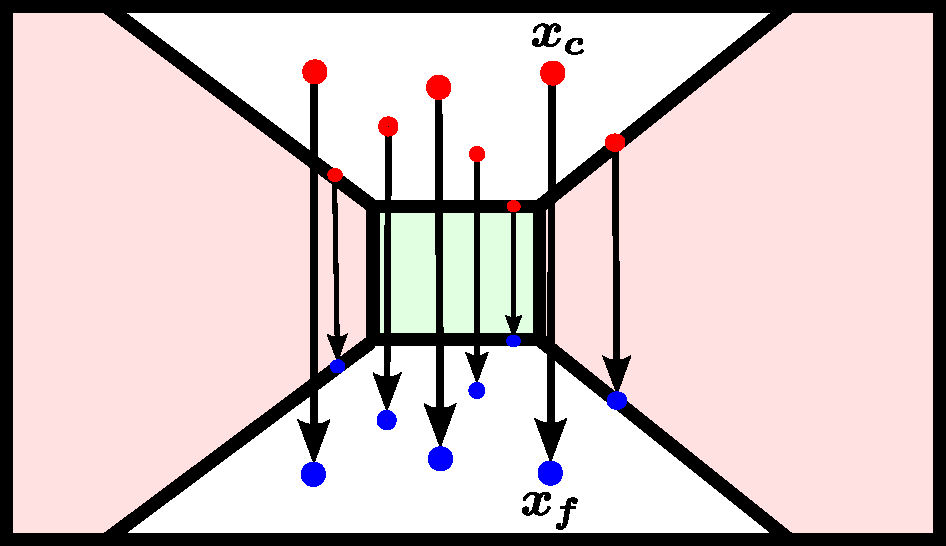
\includegraphics[width=0.5\textwidth]{manhattan_homology}
  \caption{The mapping $\Hcf$ transfers points between the ceiling
    and floor.}
  \label{fig:homology}
\end{figure}

Since the floor and ceiling planes are parallel, there is a planar
homology $\Hcf$ such that
\begin{equation}
  \FloorPt = \Hcf \CeilPt
\end{equation}
if and only if $\pfloor$ and and $\pceil$ are in correspondence
\cite{Criminisi01}. We define $\HomParam$ as the unique real number
such that
\begin{equation}
  \label{eq:manhattanhom}
  \Hcf = I + \HomParam\frac{\vvpt\horizon^T}{\vvpt \cdot \horizon}
\end{equation}
where
\begin{equation}
  \horizon = \CamMatrix\CamR\ex \cross \CamMatrix\CamR\ey
\end{equation}
is the horizon line. Given any corresponding pair
$(\FloorPt,\CeilPt)$, $\HomParam$ is given by \cite{Criminisi01}
\begin{equation}
  \HomParam = 
  \langle\vvpt,\CeilPt,\FloorPt,(\CeilPt\times\FloorPt)\times\horizon\rangle ~,
\end{equation}
where
\begin{equation}
  \langle \vect{a},\vect{b},\vect{c},\vect{d} \rangle = \frac{
    (\vect{a}-\vect{c}) \cdot (\vect{b}-\vect{d})
  }{
    (\vect{b}-\vect{c}) \cdot (\vect{a}-\vect{d})
  }
\end{equation}
is the characteristic cross ratio of $\Hcf$.

Note that $\HomParam$ is invariant to the camera intrinsics. To see
this, consider transforming the image by some homography $M$. In the
transformed image the horizon is given by
$\horizon'=|M|M^{-T}\horizon$, the vertical vanishing point is
$\vvpt'=M\vvpt$, and the Manhattan homology is
\begin{equation}
  \label{eq:homprime}
  \Hcf' = I + \HomParam'\frac{\vvpt'\horizon'^T}{\vvpt'\cdot\horizon'}~.
\end{equation}
We also have that
\begin{eqnarray}
  \Hcf' &=& M \Hcf M^{-1} \\
  &=& M (I + \HomParam\frac{\vvpt\horizon^T}{\vvpt \cdot
    \horizon})M^{-1} ~.
\end{eqnarray}
Substituting $\horizon=\frac{1}{|M|}M^T\horizon'$ and
$\vvpt=M^{-1}\vvpt'$ gives
\begin{eqnarray}
  \Hcf' &=& I + \HomParam
    \frac{M(M^{-1}\vvpt')(\frac{1}{|M|}M^T\horizon')^T M^{-1}}
         {(M^{-1}\vvpt')^T(\frac{1}{|M|}M^T\horizon')}\\
  \label{eq:comparehom}
  &=& I + \HomParam\frac{\vvpt'\horizon'^T}
                        {\vvpt'\cdot\horizon'} ~.
\end{eqnarray}
Comparing \eqnref{comparehom} and \eqnref{homprime} shows that
$\HomParam'=\HomParam$. We therefore assume without loss of generality
that $\CamMatrix$ is the identity for the remainder of this section.

To complete our parametrisation of the floor and ceiling planes we
need to show how to compute $(\HomParam,\ScaleParam)$ from
$(\zfloor,\zceil)$. We may simply set $\ScaleParam$ to either
$\zfloor$ or $\zceil$. Let
\begin{eqnarray}
  \efloor = \zfloor ~ \ez \\
  \eceil = \zceil ~ \ez \\
  \pfloor = \RetProj{\efloor} \\
  \pceil = \RetProj{\eceil}
\end{eqnarray}
Then
\begin{eqnarray}
  (\pceil \cross \pfloor) \cross \horizon &=&
    \bigl((\RetProj{\efloor}) \cross (\RetProj{\eceil}\bigr))
    \cross
    \bigl(\CamR\ex \cross
          \CamR\ey \bigr)\\
  &=& \bigl( (\RetProj{\eceil}) \cross (\RetProj{\efloor}) \bigr)
      \cross
      \CamR(\ex\cross\ey) \\
  &=& \bigl( \CamR(\eceil-\efloor)\cross\CamTr \bigr)
      \cross
      \CamR\ez ~.
\end{eqnarray}
We can now write
\begin{eqnarray}
  \HomParam &=& 
    \langle\vvpt,\pceil,\pfloor,(\pceil\cross\pfloor)\cross\horizon\rangle \\
  &=& \frac{
    \bigl(\vvpt-\pfloor\bigr)^T
    \bigl(\pceil-(\pceil\cross\pfloor)\cross\horizon\bigr)
   }{
    \bigl(\pceil-\pfloor\bigr)^T
    \bigl(\vvpt-(\pceil\cross\pfloor)\cross\horizon\bigr)
   }\\
  &=& \frac{
    \bigl(\CamR\ez - (\CamR\efloor+\CamTr)\bigr)^T
    \bigl(\CamR\eceil+\CamTr-
          (\CamR(\eceil-\efloor)\cross\CamTr)\cross\CamR\ez
          \bigr)
   }{
    \bigl(\CamR\eceil+\CamTr-\CamR\efloor-\CamTr\bigr)^T
    \bigl(\CamR\ez-
          (\CamR(\eceil-\efloor)\cross\CamTr)\cross\CamR\ez
          \bigr)
   }\\
  &=& \frac{
    \bigl(\ez - \efloor - \CamR^T\CamTr\bigr)^T R^T
    \bigl(\CamR\eceil+\CamTr-
          (\CamR(\eceil-\efloor)\cross\CamTr)\cross\CamR\ez
          \bigr)
   }{
    \bigl(\eceil-\efloor\bigr)^T R^T
    \bigl(\CamR\ez-
          (\CamR(\eceil-\efloor)\cross\CamTr)\cross\CamR\ez
          \bigr)
   }\\
  &=& \frac{
    \bigl(\ez - \efloor - \CamR^T\CamTr\bigr)^T
    \bigl(\eceil + \CamR^T\CamTr -
          ((\eceil-\efloor)\cross\CamR^T\CamTr)\cross\ez
          \bigr)
   }{
    (\eceil-\efloor)^T\ez -
    (\eceil-\efloor)^T(((\eceil-\efloor)\CamR^T\CamTr)\ez)
   }\\
  &=& \frac{
    (\ez-\efloor-\CamR^T\CamTr)^T(\eceil+\CamR^T\CamTr)
    +(\zceil-\zfloor)(\|\CamTr\|^2 - (\ez^T\CamR^T\CamTr)^2)
   }{
    \zceil-\zfloor
   }\\
  &=& \frac{1}{\zceil-\zfloor}
    \Bigl( (\zceil + \zcam)(1-\zfloor-\zcam) + \zcam^2 - \|\CamTr\|^2 \Bigr)
     + \|\CamTr\|^2 - \zcam^2
\end{eqnarray}
where in the last line we substituted $\zcam =
\ez^T\CamR^T\CamTr$.

\subsection{Parametrising walls}

We choose to parametrise $\Polyline$ in image coordinates because this
will simplify the algorithms to be presented later. We first present
the image--domain parametrisation, then show that it uniquely
specifies a 3D scene.

Consider the scenes shown in \figref{example-scenes}. Following
rectification, vertical edges in the world appear vertical in each
image, including the vertical seams between adjacent wall segments, so
any line drawn vertically from the top to bottom of a rectified image
intersects exactly one wall segment. That this is true in general
follows from our assumption that walls meet at vertical seams and
extend continuously from floor to ceiling, that the camera is located
between the floor and ceiling planes, and that the environment is
closed.

\begin{figure}[tb]%
  \centering
    \begin{tabular}{ccc}
      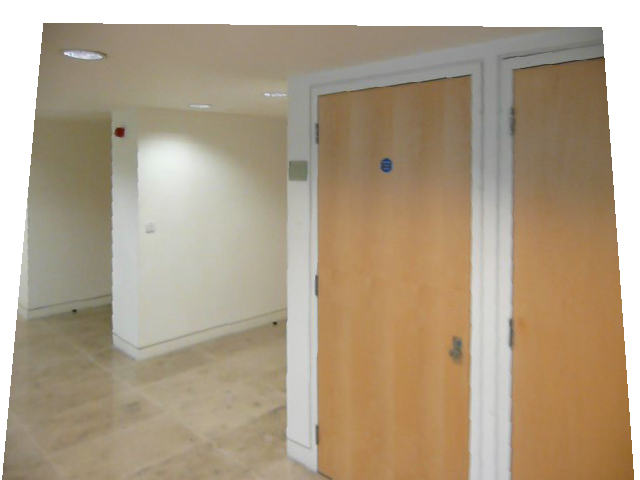
\includegraphics[width=0.3\textwidth]{true_models/lab_ground1_010_rect.png} &
      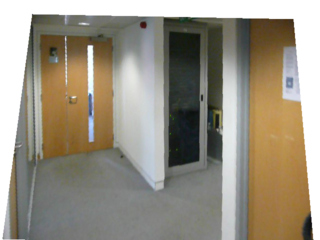
\includegraphics[width=0.3\textwidth]{true_models/lab_kitchen_030_rect.png} &
      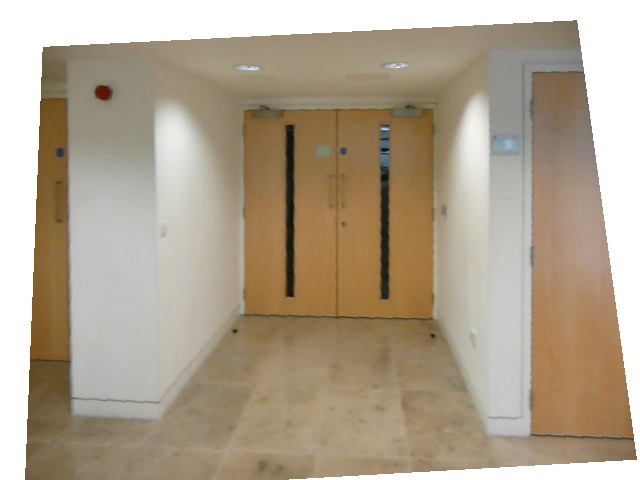
\includegraphics[width=0.3\textwidth]{true_models/lab_ground1_030_rect.png}
      \\      
      \includegraphics[width=0.3\textwidth]{true_models/lab_ground1_010} &
      \includegraphics[width=0.3\textwidth]{true_models/lab_kitchen_030} &
      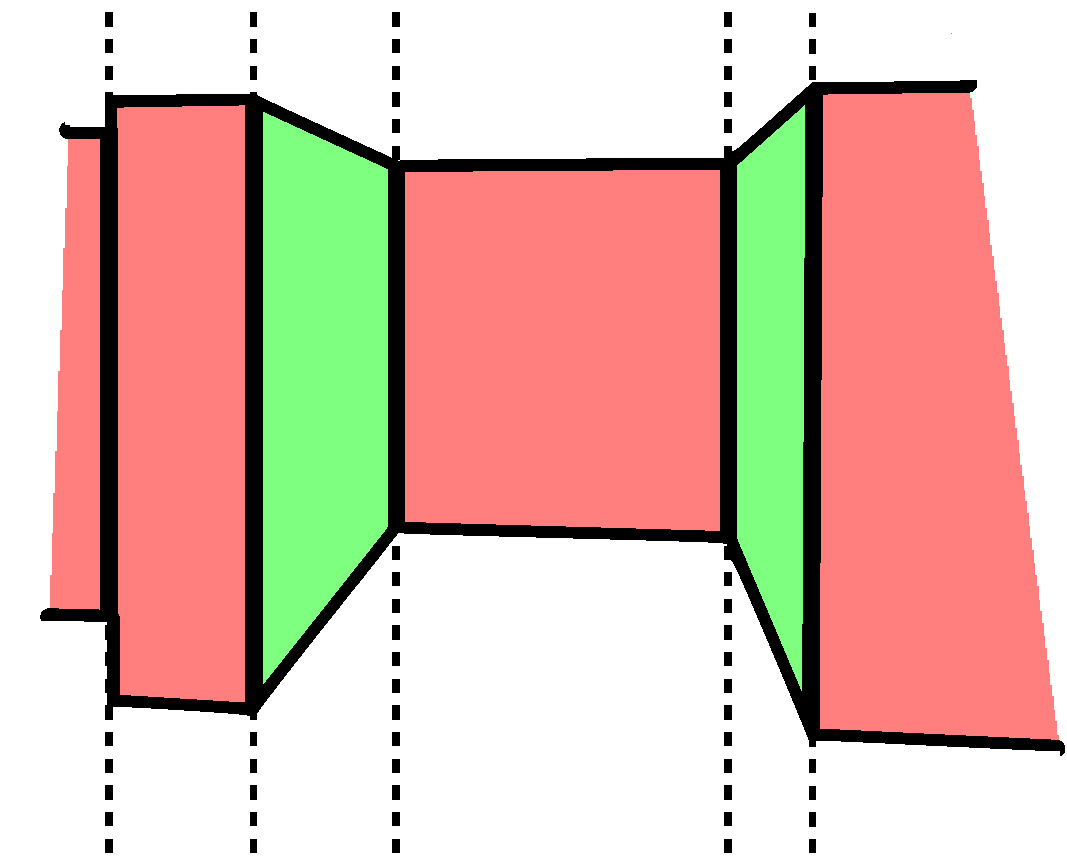
\includegraphics[width=0.3\textwidth]{true_models/lab_ground1_030}
    \end{tabular}
  \caption{Three input images and the indoor Manhattan models we
    seek. Notice how each image column intersects exactly one
    wall.}
  \label{fig:example-scenes}
\end{figure}

It turns out that once the vanishing points $\vpt_i$ and the Manhattan
homology $\Hcf$ are known, the quadrangle outlining a wall segment in
rectified image coordinates is fully specified by just four scalars,
\begin{equation}
  \label{eq:wall-def}
  \Wall = ( x_0, y, \WallOrient, x_1 )
\end{equation}
where $x_0$ is the location of the left edge, $x_1$ is the location of
the right edge, $y$ is the $y$--coordinate of the top--left corner, and
$\WallOrient\in\{1,2\}$ is the index of the vanishing point associated with
the wall. The four vertices of the wall are then given by
\begin{eqnarray}
  \label{eq:pi}
  \vect{p_i} &=& \begin{bmatrix}x&y&1\end{bmatrix}^t \\
  \label{eq:qi}
  \vect{q_i} &=& \vect{p_i}\cross\vect{v_{a}}\cross
               \begin{bmatrix}1&0&-c_{i+1}\end{bmatrix}^T\\
  \label{eq:ri}
  \vect{r_i} &=& \Hcf \vect{q_i}\\
  \label{eq:si}
  \vect{s_i} &=& \Hcf \vect{p_i} ~.
\end{eqnarray}

\begin{figure}[tb]%
  \centering
  \quad
  \includegraphics[width=0.45\textwidth]{pqrs}
  \caption{The row/column indices $c_i,c_{i+1},r_i,$ together with the
    vanishing point index $a_i\in\{l,r\}$ and the homology $\Hcf$
    fully determine the four vertices of a wall.}
  \label{fig:pqrs}
\end{figure}

\figref{pqrs} illustrates the geometry of the parametrisation
above. Since each image column intersects exactly one
wall, we may think of the scene as a sequence of walls from left to
right in the image. This observation suggests our scene
parametrisation, which is simply a sequence of wall segments. We make
the additional observation that the right edge of a wall ($x_1$ in
equation \eqnref{wall-def}) is redundant because it is always
coincident with the left edge of the wall to its right. A scene
therefore is fully specified by
\begin{equation}
  \Scene =
  ( x_1,y_1,\WallOrient_1,
   ~x_2,y_2,\WallOrient_2,
   ~\ldots,
   ~x_{n-1},y_{n-1},\WallOrient_{n-1},
   ~x_n ) ~.
  \label{eq:vertex-repr}
\end{equation}
An example scene and its parametrisation is shown in
\figref{scene-params}. Note that although the right edge of a wall
always coincides with the left edge of its neighbour, it is not always
the case that the top and bottom edges of adjacent walls meet at a
point, \ie $\vect{r_i} \neq \vect{s_{i+1}}$ in general. For example,
notice the second edge in \figref{scene-params}.

\begin{figure}[tb]
  \centering
  \includegraphics[width=0.42\textwidth]{new-model-params}
  \caption{An illustration of the model
    $\Scene=(c_1,r_1,a_1,\ldots,c_4,r_4,a_4,c_5)$.}
  \label{fig:scene-params}
\end{figure}

\subsubsection{Physical Feasibility}

Not all scenes $\Scene$ are physically realisable
as metric reconstructions, but those that are not can be discarded
using simple tests on the locations of walls and vanishing points as
enumerated by Lee \etal \cite{Lee09}. The reader is referred to their
paper for details; the key result for our purposes is that a model is
feasible if all of its corners are feasible, and the feasibility of a
corner is dependent only on the immediately adjoining walls. We
discuss these issues in detail during \chapref{inference}.

\subsection{The Seam Representation}
\label{sec:seam-representation}

\begin{figure}[tb]%
  \centering
  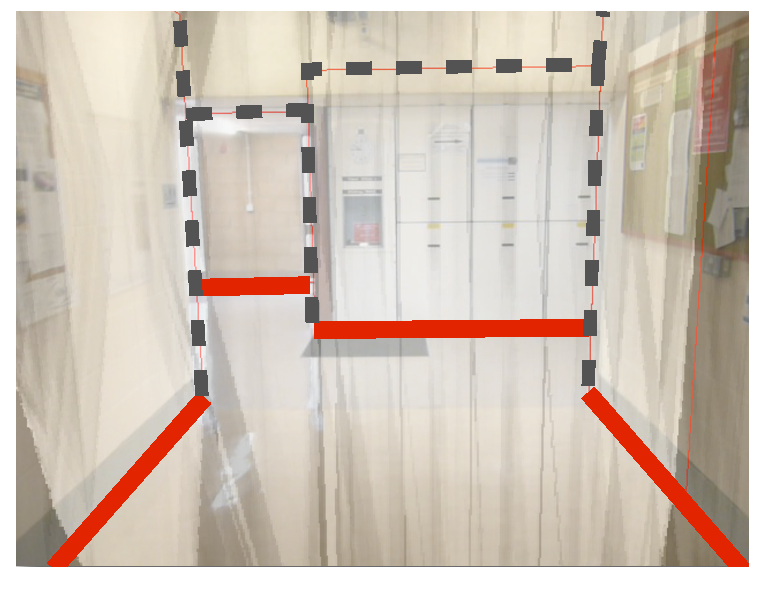
\includegraphics[width=0.6\textwidth]{seam-example}
  \caption{An example of an indoor Manhattan scene and its seam
    representation shown in red. The grey dotted lines can be
    recovered from the seam using the Manhattan homology $\Hcf$.}
  \label{fig:seam-example}
\end{figure}

For the purpose of the probabilistic model that we will present in
chapter \chapref{inference} we will now present an additional, slightly
different parametrisation that we will refer to as the \textit{seam}
representation of indoor Manhattan scenes. We will refer to the
parametrisation of equation \eqnref{vertex-repr} as the
\textit{vertex} representation. A scene in vertex representation
$\Scene$ uniquely determines a scene in seam $\Seam$ representation,
but the converse is not true. For this reason we will always work in
the vertex representation during inference, but to evaluate
likelihoods, priors, and posteriors for a fixed scene we will find it
notationally more convenient to work in the seam representation. Under
the seam representation a scene is represented by associating a pair of
scalars $(\seam_j,\WallOrient_j)$ to each image column $j$,
\begin{equation}
  \label{eq:seam-def}
  \Seam = \{(\seam_j,\WallOrient_j)\}_{j=0}^\Width  ~,
\end{equation}
where $\seam_j$ is the $y$--coordinate of the bottom edge of the wall
that intersects the $j$\th column, and $\WallOrient_j\in\{1,2\}$ is
the index of its associated vanishing point. Note that the size of
this representation is proportional to the image width, whereas the
size of the vertex representation is proportional to the number of
distinct wall segments. See \figref{seam-example}
for an illustration of this parametrisation.

We compute the seam representation $\Seam$ from a scene in vertex
representation $\Scene$ as follows. For each $j\in[0,\Width]$ we
identify the index of the (unique) wall segment that intersects column
$j$ by finding $x_i,x_{i+1}\in\Scene$ such that $x_i \leq j \leq
x_{i+1}$. Next we compute $\vect{s_i}$ and $\vect{r_i}$ according to
equations \eqnref{si} and \eqnref{ri}, after which the position of the
wall seam at column $j$ is given by
\begin{equation}
  \label{eq:seam-from-scene}
  \seam_j = (\vect{r_i} \cross \vect{s_i}) \cross
  \begin{bmatrix} 0 & 1 & -j \end{bmatrix}^T ~.
\end{equation}
Finally, the orientation $\WallOrient_j$ at column $j$ is equal to the
orientation of the identified wall segment, $\WallOrient_i$. The
constructive process described above shows that there is exactly one
seam $\Seam$ associated with a scene in vertex
representation. However, there is no unique mapping in the reverse
direction. In other words, the mapping from vertex representation to
seam representation is many--to--one.

%%%%%%%%%%%%%%%%%%%%%%%%%%%%%%%%%%%%%%%%%%%%%%%%%%%%%%%%%%%%%%%%%%%%%%%%
\section{Deductions}
\label{sec:misc-geometry}

In this section we make several geometric observations that are
crucial to the following chapters.

\subsection{Classification of Corners}
\label{sec:corner-categories}

\begin{figure}[tb]%
  \centering
  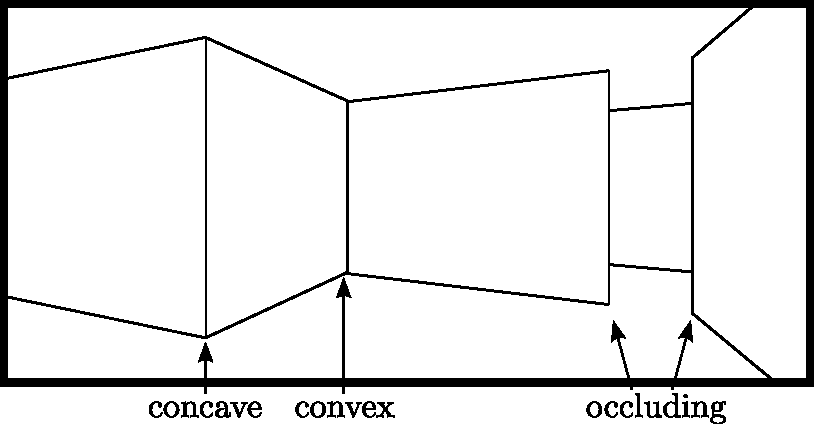
\includegraphics[width=0.6\textwidth]{corner-types}
  \caption{Each corner in an indoor Manhattan environment can be
    categorised as concave, convex, or occluding.}
  \label{fig:corner-types}
\end{figure}

Lee \etal \cite{Lee09} showed that corners between adjacent walls
can be divided into three categories as follows.
\begin{itemize}
  \item{A \textit{convex corner} occurs where two wall segments meet
    exactly and form an internal angle not greater than $180\degrees$, \ie
    \begin{eqnarray}
      \vect{r_i} &=& \vect{s_{i+1}}\\
      &\mbox{and}&\\
      \frac{(\vect{s_i}-\vect{r_i})\cdot(\vect{q_i}-\vect{r_i})}
           {\|\vect{s_i}-\vect{r_i})\|\|(\vect{q_i}-\vect{r_i}\|}
      &\leq&
      \frac{(\vect{r_{i+1}}-\vect{r_i})\cdot(\vect{q_i}-\vect{r_i})}
           {\|\vect{r_{i+1}}-\vect{r_i})\|\|(\vect{q_i}-\vect{r_i}\|} ~.
    \end{eqnarray}
  }
  \item{A \textit{concave corner} occurs where two wall segments meet
    exactly and form an internal angle greater than $180\degrees$, \ie
    \begin{eqnarray}
      \vect{r_i} &=& \vect{s_{i+1}}\\
      &\mbox{and}&\\
      \frac{(\vect{s_i}-\vect{r_i})\cdot(\vect{q_i}-\vect{r_i})}
           {\|\vect{s_i}-\vect{r_i})\|\|(\vect{q_i}-\vect{r_i}\|}
      &>&
      \frac{(\vect{r_{i+1}}-\vect{r_i})\cdot(\vect{q_i}-\vect{r_i})}
           {\|\vect{r_{i+1}}-\vect{r_i})\|\|(\vect{q_i}-\vect{r_i}\|} ~.
    \end{eqnarray}
  }
  \item{An \textit{occluding corner} occurs where two wall segments
    meet but their lower edges do not coincide, \ie
    \begin{equation}
      \vect{r_i} \neq \vect{s_{i+1}}
    \end{equation}
  }
\end{itemize}
Examples of each type of corner are shown in \figref{corner-types}.

\subsection{Recovering Metric Scene Structure}
\label{sec:metric-recovery}

We now show that once $\SceneR$ and $\Zs$ are known, a scene $\Scene$
in vertex representation uniquely specifies a 3D scene
$\Reconstruction$. We show this by demonstrating how to convert a
scene $\Scene$ to a floorplan $\Floorplan$, after which we may apply
equations \eqnref{pi}, \eqnref{qi}, \eqnref{ri}, and \eqnref{si} to
recover a polygonal reconstruction.

Let $\backproj(\Pixel;\vect{w},\CamMatrix,\CamR,\CamTr)$ be the
back--projection of image point $\Pixel$ onto the plane
$\vect{x}\cdot\vect{w}=0$ given camera intrinsics $\CamMatrix$ and
extrinsics $\CamR,\CamTr$. To compute this we solve for $\vect{y}$ in
\begin{eqnarray}
  P \vect{y} &=& \vect{0}\\
  \| \vect{y} \| &=& 1
\end{eqnarray}
where
\begin{equation}
  P =
  \begin{bmatrix}
    & \CamMatrix\CamR & & \CamMatrix\CamTr-\Pixel \\
    0 & 0 & 1 & -\zfloor
  \end{bmatrix}~.
\end{equation}
We will usually omit the camera parameters and simply write
$\backproj(\Pixel;\vect{w})$. Furthermore, since we will often be
back--projecting onto planes orthogonal to the $z$ axis we adopt the
short--hand
\begin{equation}
  \backproj(\Pixel;z) = \backproj(\Pixel;
    \begin{bmatrix}0 & 0 & 1 & -z\end{bmatrix}) ~.
\end{equation}

To recover a floorplan $\Floorplan$ from a scene $\Scene$ we simply
need to back--project $\vect{q_i},\vect{s_i}$ pairs onto the floor
plane. This is formalised in \algref{scene-to-recon}.

\begin{algorithm}
  \begin{algorithmic}
    \REQUIRE{$\Scene =(x_1,y_1,\WallOrient_1,\ldots,x_n)$ ~~~
      \{a scene in vertex representation\}}
    \ENSURE $\Floorplan=\{(\vect{u_i},\vect{v_i})\}$
    \STATE{$\Floorplan \leftarrow \emptyset$}
    \FOR{$i=1 \ldots n-1$}
      \STATE{$\vect{u_i}=\backproj(\vect{s_i}; \zfloor)$}
      \STATE{$\vect{u_i}=\backproj(\vect{r_i}; \zfloor)$}
      \STATE{$\Floorplan \leftarrow \Floorplan \union (\vect{u_i},\vect{v_i})$}
    \ENDFOR
  \end{algorithmic}
  \caption{\label{alg:scene-to-recon}
    Recovering a metric 3D scene from the vertex representation
    $\Scene$.}
\end{algorithm}

\subsection{Recovering Orientation and Depth}
We say that an indoor Manhattan scene $\Scene$ predicts the depth
$\Depth_{\Pixel}$ of each pixel $\Pixel$ because we can compute the
depth of each $\Pixel$ given the hypothesis $\Scene$. Similarly, a
scene predicts an orientation $\Orient_{\Pixel}\in\SetOfOrients$ for
each image point, which is the orientation of the 3D surface that
projects to $\Pixel$.

To compute either the orientation $\Orient_{\Pixel}$ or depth
$\Depth_{\Pixel}$ for an image point $\Pixel$ we first need to
identify a wall that contains $\Pixel$ within its (image--domain)
outline. If there is such a wall then $\Pixel$ has the orientation of
that wall and we back--project $\Pixel$ onto the wall in 3D to recover
depth. If $\Pixel$ is not contained by any wall then $\Pixel$ must be
on the floor or ceiling and therefore has the horizontal
orientation. In this case we recover depth by back--projecting onto
the floor or ceiling plane, according to whether $\Pixel$ is above or
below the horizon. This process is formalised in
\algref{computing-from-scene}.

\begin{algorithm}[tb]
  \begin{algorithmic}
    \REQUIRE{$\Scene =(x_1,y_1,\WallOrient_1,\ldots,x_n)$ ~~~ 
       \{a scene in vertex representation\}}
    \REQUIRE $\Pixel=(x,y)\in\Rtwo$
    \REQUIRE $x_1 \leq x < x_n$
    \ENSURE{$i_{\Pixel} \in [1,n],
      \Orient_{\Pixel} \in \SetOfOrients,
      \Depth_{\Pixel}>0$}
    \FOR{$i = 1 \ldots n-1$}
      \IF{$x_i \leq x < x_{i+1}$}
        \STATE\COMMENT{Compute the floor--wall and ceiling--wall
          seam in column $x$}
          % TODO: euclidean projection needed below!!
        \STATE{$\seam_f \leftarrow \ey \cdot (\vect{s_i}
          \cross \vect{r_i})
          \cross \begin{bmatrix}1&0&-x\end{bmatrix}^T$}
        \STATE{$\seam_c \leftarrow \ey \cdot (\vect{s_i}
          \cross \vect{r_i})
          \cross \begin{bmatrix}1&0&-x\end{bmatrix}^T$}
        \IF{$y < \seam_c$}
          \STATE{$\Orient_{\Pixel} \leftarrow ``vert orient''$}
          \STATE{$X_{\Pixel} \leftarrow \backproj(\Pixel; \zceil)$}
        \ELSIF{$\seam_c < y < \seam_f$}
          \STATE{$\Orient_{\Pixel} \leftarrow \WallOrient_x$}
          \STATE{$w_{\Pixel} \leftarrow
            \begin{bmatrix}
              1 & 0 & 0 & -\backproj(\vect{x_f}; \zfloor)\cdot\ex
            \end{bmatrix}^T$}
          \STATE{$X_{\Pixel} \leftarrow \backproj(\Pixel; w_{\Pixel})$}
        \ELSE
          \STATE{$\Orient_{\Pixel} \leftarrow ``vert orient''$}
          \STATE{$X_{\Pixel} \leftarrow \backproj(\Pixel; \zfloor)$}
        \ENDIF
        \STATE{$\Depth_{\Pixel} \leftarrow
          (\CamR X_{\Pixel} + \CamTr) \cdot \ez$}
        \RETURN
      \ENDIF
    \ENDFOR
  \end{algorithmic}
  \caption{\label{alg:computing-from-scene}
    Recovering orientation and depth for an image location
    $\Pixel$ under a scene hypothesis $\Scene$.}
\end{algorithm}

These calculations are considerably simpler in the seam
representation, which is why it proves useful in following
chapters. Suppose we are given a scene in seam representation $\Seam$
and an integer pixel location $\Pixel\in\Ints^2$. We first look up the
the pair $(\seam_j,\WallOrient_j)\in\Seam$ for the column $j$ in which the
pixel $\Pixel=(x,y)$ falls, which we denote
$(\seam_x,\WallOrient_x)$. Then the floor--wall seam in column
$x$ is at $\seam_f=\seam_x$ and the ceiling--wall seam
can be recovered using the Manhattan homology. From here the
orientation and depth at $\Pixel$ are obtained using the procedure
shown in \algref{seam-depth-orient}.

\begin{algorithm}[tb]
  \begin{algorithmic}
    \REQUIRE{$\Seam = \{(\seam_j,\WallOrient_j)\}$ ~~~
      \{a scene in seam representation\}}
    \REQUIRE{$\Pixel=(x,y)\in\Ints^2$ ~~~
      \{a query pixel\}}
    \ENSURE{$\Orient_{\Pixel} \in \SetOfOrients,
      \Depth_{\Pixel}>0$}
    \STATE\COMMENT{Compute the floor--wall and ceiling--wall
      seam in column $x$}
    \STATE{$\seam_f \leftarrow \seam_{x}$}
    \STATE{$\vect{x_f} \leftarrow
      \begin{bmatrix}
        x & \seam_f & 1
      \end{bmatrix}^T$}
    \STATE{$\vect{x_c} \leftarrow \Hcf \vect{x_f}$}
    \STATE{$\seam_c \leftarrow \frac{\vect{x_c}\cdot\ey}
      {\vect{x_c}\cdot\ez}$}
    \IF{$y < \seam_c$}
      \STATE{$\Orient_{\Pixel} \leftarrow ``vert orient''$}
      \STATE{$X_{\Pixel} \leftarrow \backproj(\Pixel; \zceil)$}
    \ELSIF{$\seam_c < y < \seam_f$}
      \STATE{$\Orient_{\Pixel} \leftarrow \Orient_x$}
      \STATE{$\vect{w}_{\Pixel} \leftarrow
        \begin{bmatrix}
          1 & 0 & 0 & -\backproj(\vect{x_f}; \zfloor)\cdot\ex
        \end{bmatrix}^T$}
      \STATE{$X_{\Pixel} \leftarrow \backproj(\Pixel; \vect{w}_{\Pixel})$}
    \ELSE
      \STATE{$\Orient_{\Pixel} \leftarrow ``vert orient''$}
      \STATE{$X_{\Pixel} \leftarrow \backproj(\Pixel; \zfloor)$}
    \ENDIF
    \STATE{$\Depth_{\Pixel} \leftarrow
      (\CamR X_{\Pixel} + \CamTr) \cdot \ez$}
  \end{algorithmic}
  \caption{\label{alg:seam-depth-orient}
    Recovering orientation and depth for an
    image location $\Pixel$ under the seam representation $\Seam$.}
\end{algorithm}

\subsection{Column--wise Decomposability}
\label{sec:col-decomposability}

We have so far shown that the vertex representation suffices to
recover metric scene structure up to scale, and that the depth and
orientation predicted for each pixel can be computed directly from
either the vertex or seam representation. One property of particular
significance for the algorithms to be presented in the remainder of
this thesis is that the procedure of \algref{seam-depth-orient} only
requires access to the pair $(\seam_j,\WallOrient_j)$ for the image
column $j$ that contains the query pixel. That is, the depth and
orientation predicted for a pixel $\Pixel$ are functionally
independent of the location of the floor--wall seam in columns other
than the one containing $\Pixel$.

%%%%%%%%%%%%%%%%%%%%%%%%%%%%%%%%%%%%%%%%%%%%%%%%%%%%%%%%%%%%%%%%%%%%%%%%
\section{Conclusion}

We have presented the indoor Manhattan model, in which the world is
represented by floor, ceiling, and wall planes. We have motivated this
model in terms of its salience, compactness, and the simple
parametrisations it permits. The vertex and seam representations are
the primary contributions of this chapter; their specific structure is
crucial to all following chapters. In particular, we will make
repeated use of the decomposability property described in
\secref{col-decomposability}. While this chapter has described the
geometry of ideal indoor Manhattan environments, the system that we
develop in this thesis is not restricted to working in such sterile
contexts; rather, the model presented in this chapter describes the
scene structure that we seek to recover \textit{despite} clutter and
sensor noise.
